
\section{Mezclando k vectores ordenados}

\subsection{Automatización}
\begin{frame}{Scripts}
	\begin{block}{Script}
		Podemos obtener los datos fijando el n\'umero de vectores usados.
	\end{block}
	
	\begin{exampleblock}{script.sh}
	g++ -std=c++11 ../src/mezcla.cpp

	nelementos=10

	while [ \$nelementos -lt 2500 ]; do
    
    		./a.out \$nelementos 200 3
    
    		let nelementos=nelementos+25
	
	done
	\end{exampleblock}
\end{frame}

%%%%%%%%%%%%%%%%%%%%%%%%%%%%%%%%%%%%%%%%%%%%

\begin{frame}
	\begin{block}{Script}
		Si queremos fijar el n\'umero de vectores usaremos
	\end{block}
	
	\begin{exampleblock}{script.sh}
	kvectores=10

	while [ \$kvectores -lt 2500 ]; do
    
    		./a.out 200 \$kvectores 2
    	
    		let kvectores=kvectores+25

	done
	\end{exampleblock}
\end{frame}

%%%%%%%%%%%%%%%%%%%%%%%%%%%%%%%%%%%%%%%%%%%%

\begin{frame}
	\begin{block}{Script}
	Datos en 3 dimensiones, número de vectores, elementos del vector, y tiempo del algoritmo
	\end{block}
	
	\begin{exampleblock}{script.sh}
	nelementos=10

	nvectores=10

	while [ \$nelementos -lt 1000 ]; do
   	
   		./a.out \$nelementos 10 1
      		
   		...
   		
   		./a.out \$nelementos 910 1

   		let nelementos=nelementos+100
	done
	\end{exampleblock}
\end{frame}

%%%%%%%%%%%%%%%%%%%%%%%%%%%%%%%%%%%%%%%%%%%%

\begin{frame}{Scripts de gnuplot}
	\begin{block}{Gnuplot}		
		Los datos están en "datos.dat". Ejecutamos	
			
		\hspace{1cm}\$ gnuplot algoritmo.gp
	\end{block}
	\pause
	
	\begin{columns}

	\begin{column}{5cm}
	\begin{exampleblock}{algoritmo.gp}
	set terminal pngcairo
	
	set output "grafica.png"

	set title "..."

	set xlabel "Vectores/Elementos del vector"

	set ylabel "Tiempo (s)"

	set fit quiet

	f(x) = ...

	fit f(x) "datos.dat" via a

	plot "datos.dat", f(x)
	\end{exampleblock}
	\end{column}
	\pause
	
	\begin{column}{5cm}
	\begin{block}{Funciones ajustadas}
		\[f(x) = a*x\]
		\[g(x) = a*x*x\]
		\[h(x) = a*x*(log(200)/log(2))\]
	\end{block}
	\end{column}
	
	\end{columns}
\end{frame}

%%%%%%%%%%%%%%%%%%%%%%%%%%%%%%%%%%%%%%%
\subsection{Ordenador usado}
\begin{frame}{Ordenador usado}
	\begin{alertblock}{Ordenador usado para la ejecuci\'on}
	HP Pavilion g series (Pavilion g6)

	Sistema operativo: ubuntu 14.04 LTS

	Memoria: 3.8 GiB (4Gb)

	Procesador: Inter Core i3-2330M CPU @ 2.20GHz x 4

	Gráficos: Intel Sandybridge Mobile

	Tipo de SO: 64 bits

	Disco: 487.9 GB	
	\end{alertblock}
\end{frame}


%%%%%%%%%%%%%%%%%%%%%%%%%%%%%%%%%%%%%%

\begin{frame}{Problema}
	\begin{block}{Mezclando k vectores ordenados}
	Se tienen $k$ vectores ordenados (de menor a mayor), cada uno con $n$ elementos, y 				queremos combinarlos en un único vector ordenado (con $kn$ elementos)
	\end{block}

	\begin{block}{Cota superior}
	Es posible imponer una cota superior teórica. Teniendo en cuenta que hay kn elementos, 	si aplicásemos un algoritmo 	de ordenación con eficiencia $O(n) = nlog(n)$ deducimos 			que podemos encontrar un algoritmo de ordenación básica con eficiencia $O(k, n) = 
	nklog(nk)$. Tomar los $k$ vectores como uno solo no aprovecha aún el hecho de que 			partes del vector están ordenadas.
	\end{block}
\end{frame}

%%%%%%%%%%%%%%%%%%%%%%%%%%%%%%%%%%%%%%%
\subsection{Fuerza bruta}
\begin{frame}{Fuerza bruta}
	\begin{block}{Algoritmo}
	En cada paso elegimos el mínimo de los primeros elementos de los $k$ vectores, será el 	primer elemento del vector creciente resultante.
	Para el siguiente paso descartamos ese elemento y calculamos otra vez el mínimo, lo 			insertamos al final del vector resultante y así sucesivamente.

	Buscar el mínimo es $O(k)=k$ ya que el vector de índices tiene $k$ 							elementos, y lo repetimos $kn$ veces.
	\end{block}
	
	\begin{block}{Eficiencia}
	\[\sum_{i=1}^{kn}k = nk^2 \implies \ O(k,n)=nk^2\]
	\end{block}
\end{frame}

%%%%%%%%%%%%%%%%%%%%%%%%%%%%%%%%%%%%%%%%
\subsection{Divide y vencerás}
\begin{frame}{Divide y vencerás}
	\begin{block}{Algoritmo}
	Usaremos mergesort, pero con los primeros montículos ya creados, por tanto tendrá una 		constante oculta menor que usar mergesort para $kn$ datos arbitrarios. 
	
	En el proceso lo que haremos es ir mezclando las partes de dos en dos. El algoritmo 			que mezcla dos vectores en un único tiene eficiencia $O(n) = n$.
	\end{block}
\end{frame}

\begin{frame}
	\begin{block}{Código} % errorl
		\begin{figure}[h]
    		\centering
    		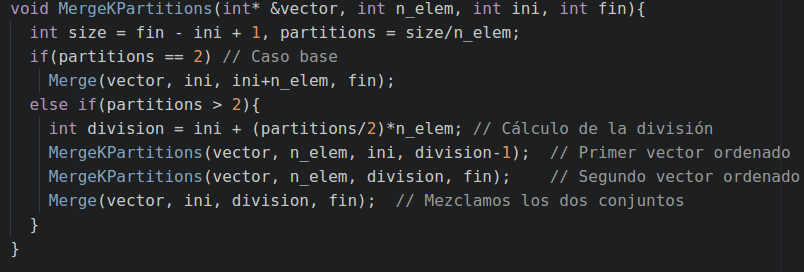
\includegraphics[width=0.9\textwidth]{./Imagenes/dyv.png}
    		\label{fig:mesh1}
		\end{figure}
	\end{block}
\end{frame}

%%%%%%%%%%%%%%%%%%%%%%%%%%%%%%%%%%%%%

\begin{frame}
	\begin{block}{Eficiencia}
	Donde $k$ es el n\'umero de vectores y $n$ el n\'umero de elementos de cada vector:s

	\[T(k,n) = \left \{ 
	\begin{matrix} 
		2n & 				\mbox{si } k=2
	\\ 2T(k/2,n) + kn & 		\mbox{si } k>2
	\end{matrix}
	\right.\]
	\end{block}
\end{frame}

\begin{frame}
	\begin{block}{Desarrollo}
	Sustituyendo $k=2^m \implies$ $T(2^m, n) = 2T(2^{m-1}, n) + 2^mn$
	\[T(2^m, n) = 2\left[ T(2^{m-2}, n) + 2^{m-1}n \right] + 2^mn\]
	\begin{center}
	Para el caso gen\'erico, con $j \in \left[0,m-1\right] \cap\mathbb{N}$ y 						desarrollando:
	\end{center}
	\[T(2^m, n)	= 2^jT(2^{m-j}, n) + \sum_{i=1}^{m-1} 2^mn\]
	\[T(2^m, n) = 2^{m-1} T(2, n) + \sum_{i=1}^{m-1} 2^mn\]
	\[T(2^m, n) = 2^mn + (m-1) 2^mn = 2^mn[1+(m-1)] = 2^mnm\]
	\end{block}
\end{frame}

\begin{frame}{Eficiencia final}
	\begin{block}{Solución}
	Deshacemos el cambio de variable, $k=2^m \implies log_2(k)=m$:
	\[T(k,n) = knlog_2k\]
	\end{block}
\end{frame}

\subsection{Estudio emp\'irico e h\'ibrido fuerza bruta}
\begin{frame}{Ajuste fuerza bruta}
	\begin{block}
	
	Vamos a variar el n\'umero de vectores, la funci\'on que debemos ajustar es 
	$f(x) = ax^2$
	$\centering$
	
	%\fcolorbox{gray75}{gray97}{
		$a               = 1.77962\cdot 10^{-6}$
	%}
	
	Para calcular los coeficientes de correlaci\'on hemos usado la función stats de gnuplot:
	\end{block}
	
\end{frame}


\begin{frame}{Variando vectores}
	\begin{exampleblock}{Imagen}
	\begin{figure}[htb] 
	\centering
	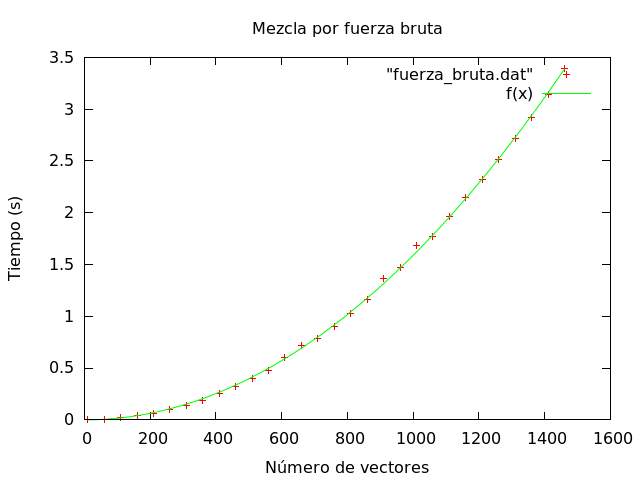
\includegraphics[width=0.7\textwidth]														{../Obligatorio/Graficas/fuerza_bruta_kvectores.png}
	\caption{Fuerza bruta con 200 elementos cada vector} 
	\label{fig:f_kvectores} 
	\end{figure}
	\end{exampleblock}
\end{frame}

\begin{frame}
	\begin{block}
	
	Para la parte en la que cambiamos el n\'umero de elementos ajustamos la funci\'on 
	$f(x) = ax$ ya 	que en $T(k, n) = nklog_2k, \ klog_2k$ es una constante, concretamente 	$200$.

	\begin{center}
	$a               = 0.00031202$

	Correlation:  $r = 0.9934$
	\end{center}
	\end{block}
\end{frame}


\begin{frame}{Imagen}
	\begin{exampleblock}
	
	\begin{figure}[h] 
	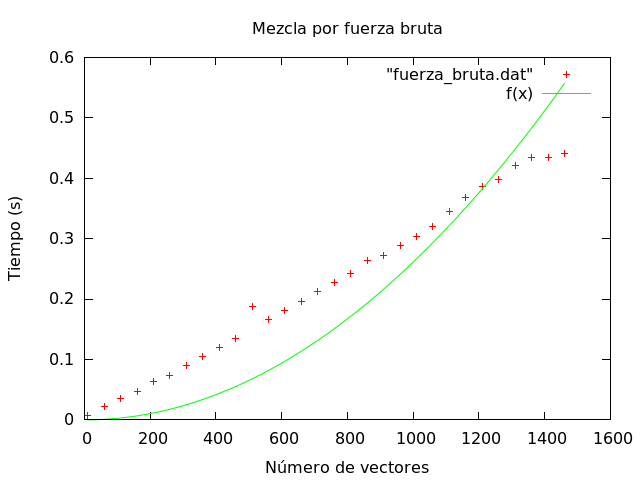
\includegraphics[width=0.7\textwidth]
	{../Obligatorio/Graficas/fuerza_bruta_nelementos.png}
	\caption{Fuerza bruta con 200 vectores} 
	\end{figure}
	
	\end{exampleblock}
\end{frame}


\subsection{Mezcla con divide y vencer\'as}
\begin{frame}[Divide y vencerás]
	\begin{block}

	La funci\'on ajustada ha sido $f(x) = ax(log(x)/log(2))$

	\begin{center}	
	$a               = 4.52594\cdot 10^{-6}$
	Correlation:  $r = 0.9863$
	\end{center}
	\end{block}
\end{frame}

\begin{frame}[Imagen]
	\begin{block}
	
	\begin{figure}[h] 
	\centering
	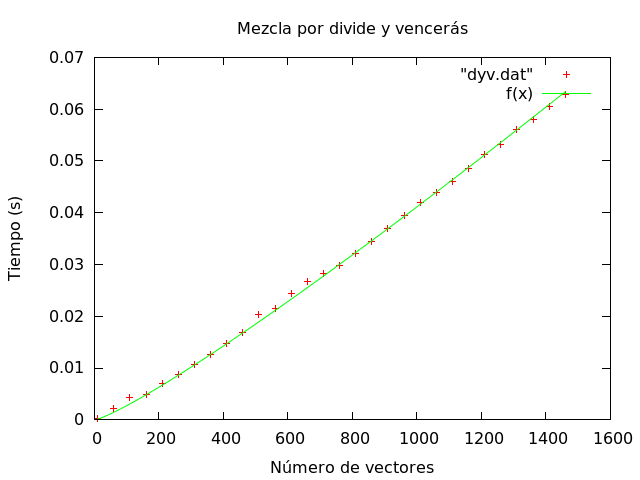
\includegraphics[width=0.7\textwidth]{../Obligatorio/Graficas/dyv_kvectores.png}
	\caption{Divide y vencerás con 200 elementos cada vector} 
	\end{figure}
	
	\end{block}
\end{frame}

\begin{frame}
	\begin{block}
	
	Si ahora fijamos $k=200$ y hacemos variable el n\'umero de elementos debemos ajustar 			la funci\'on $f(x) = ax(log(200)/log(2))$

	\begin{center}
	$a               = 3.03036\cdot 10^{-6}$
	Correlation:  $r = 0.9933$
	\end{center}
	\end{block}
\end{frame}

\begin{frame}{Imagen}
	\begin{block}{ }
	
	\begin{figure}[h] 
	\centering
	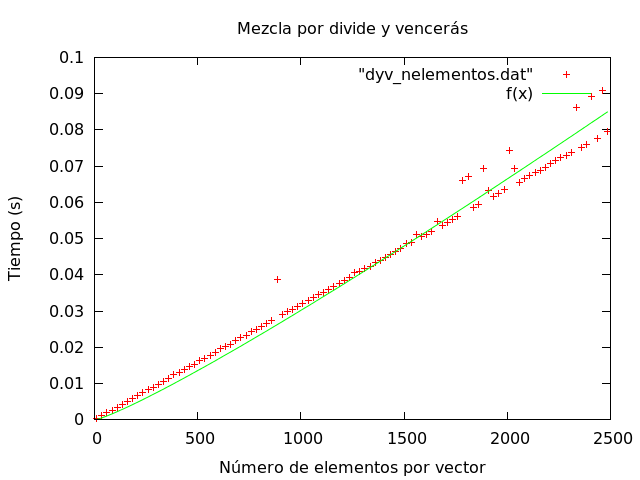
\includegraphics[width=0.7\textwidth]{../Obligatorio/Graficas/dyv_nelementos.png}
	\caption{Divide y venceras con 200 vectores} 
	\label{fig:d_nelementos} 
	\end{figure}
	
	\end{block}
\end{frame}


\subsection{Comparativa}
\begin{frame}{Según el número de vectores}
	\begin{block}
	
	\begin{figure}[htb] 
	\centering
	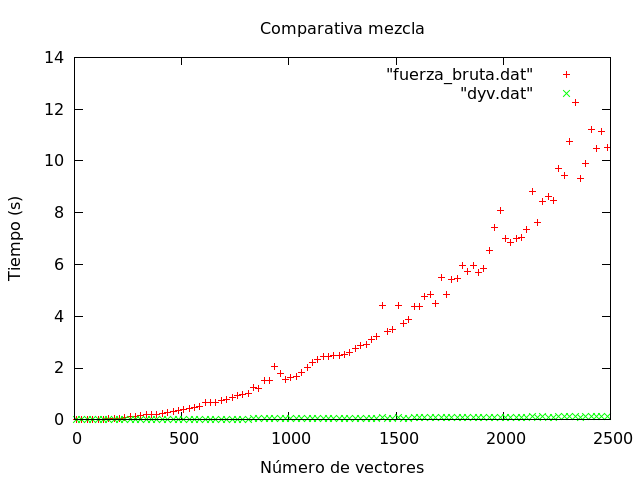
\includegraphics[width=0.7\textwidth]														{../Obligatorio/Graficas/comparativa_kvectores.png}
	\caption{Comparativa con 200 elementos cada vector} 
	\label{fig:comp_kvectores} 
	\end{figure}
	\end{block}
\end{frame}




\begin{frame}{Según el número de elementos de cada vector}
	\begin{block}
	
	\begin{figure}[htb] 
	\centering
	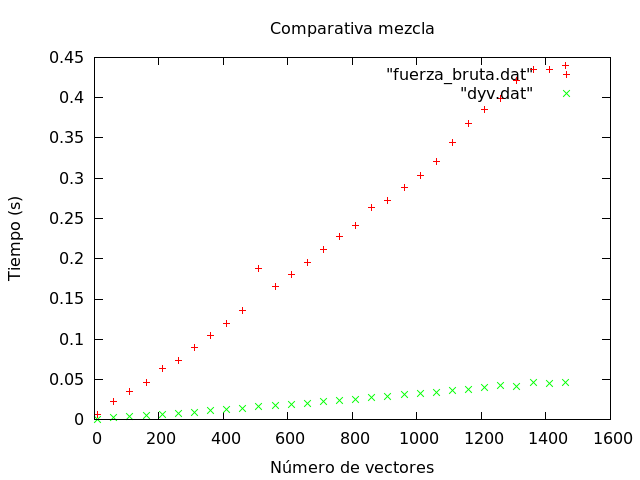
\includegraphics[width=0.7\textwidth]														{../Obligatorio/Graficas/comparativa_nelementos.png}
	\caption{Comparativa con 200 vectores} 
	\label{fig:comp_nelementos} 
\end{figure}
	\end{block}
\end{frame}


\begin{frame}
	\begin{block}
	
	Si queremos combinar los resultados podemos variar simult\'aneamente el n\'umero de 			vectores y los elementos del vector tenemos que crear gr\'aficas en $3$ dimensiones.
	De esta forma podemos comprobar que el n\'umero de vectores es un factor m\'as 				influyente que el n\'umero de elementos de cada vector. Sin embargo este es un dato 			que se aprecia en el algoritmo por fuerza bruta, en el divide y vencer\'as apenas se 			nota diferencia.
	\end{block}
\end{frame}

\begin{frame}
	\begin{block}
	
	\begin{figure}[htb] 
	\centering
	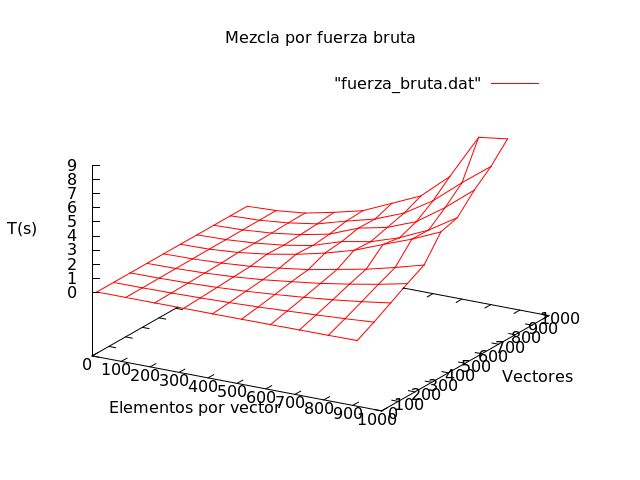
\includegraphics[width=0.7\textwidth]{../Obligatorio/Graficas/3d_fuerza_bruta.png}
	\caption{3d fuerza bruta} 
	\label{fig:3d_f} 
\end{figure}
	\end{block}
\end{frame}

\begin{frame}
	\begin{block}
	
	\begin{figure}[htb] 
	\centering
	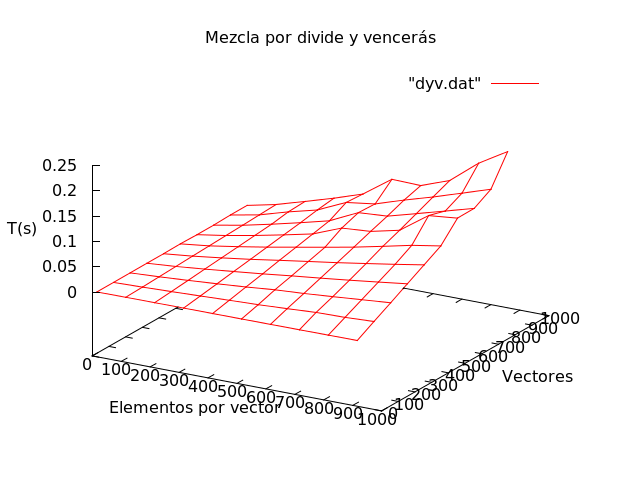
\includegraphics[width=0.7\textwidth]{../Obligatorio/Graficas/3d_dyv.png}
	\caption{3d divide y vencerás} 
	\label{fig:3d_d} 
\end{figure}
	\end{block}
\end{frame}	
